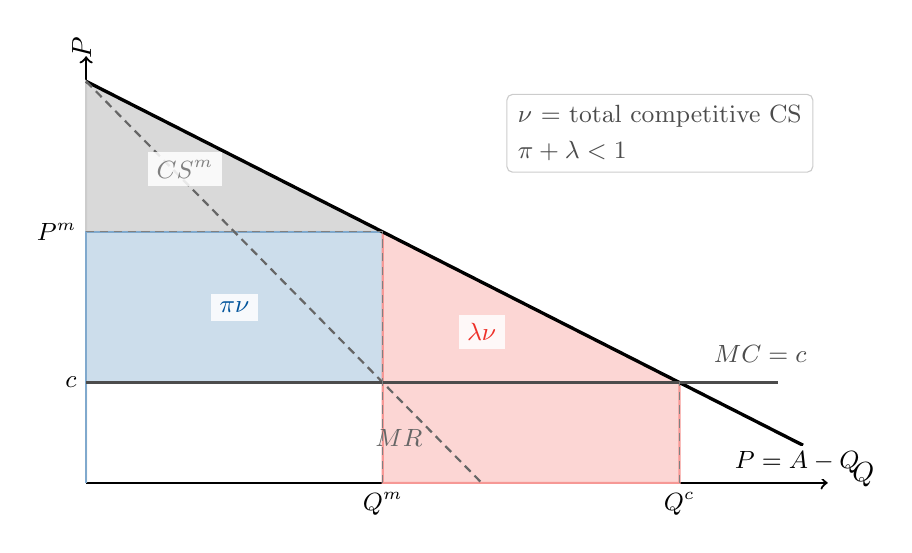
\begin{tikzpicture}
\begin{axis}[
  width=11cm, height=7cm,
  xmin=0, xmax=15,
  ymin=0, ymax=17,
  axis lines=left,
  axis line style={thick, ->},
  ticks=none,
  clip=false,
  xlabel={$Q$},
  ylabel={$P$},
  xlabel style={at={(axis description cs:1.02,0.02)}, anchor=west},
  ylabel style={at={(axis description cs:0.02,1.02)}, anchor=south},
]

% === Define colors ===
\definecolor{staBlue}{RGB}{0,83,155}
\definecolor{staRed}{RGB}{238,49,42}
\definecolor{staGreen}{RGB}{84,185,72}

% === Parameters ===
% Linear demand: P = A - Q, MC = c
% A = 16, c = 4
% Q^m = (A-c)/2 = 6, P^m = (A+c)/2 = 10
% Q^c = A - c = 12
% nu = CS under competition = (A-c)^2/2 = 72
% pi*nu = profit = (A-c)^2/4 = 36, so pi = 1/2
% lambda*nu = DWL = (A-c)^2/8 = 18, so lambda = 1/4
\pgfmathsetmacro{\A}{16}
\pgfmathsetmacro{\MC}{4}
\pgfmathsetmacro{\Qm}{(\A-\MC)/2}
\pgfmathsetmacro{\Pm}{(\A+\MC)/2}
\pgfmathsetmacro{\Qc}{\A-\MC}

% === Filled regions (BEFORE labels) ===

% Consumer surplus under monopoly (shows pi+lambda < 1)
\addplot[fill=black!15, draw=black!20, thick, forget plot]
  coordinates {(0,\Pm) (\Qm,\Pm) (0,\A)} \closedcycle;

% Profit rectangle pi*nu (blue)
\addplot[fill=staBlue!20, draw=staBlue!50, thick, forget plot]
  coordinates {(0,\MC) (\Qm,\MC) (\Qm,\Pm) (0,\Pm)} \closedcycle;

% DWL triangle lambda*nu (red)
\addplot[fill=staRed!20, draw=staRed!50, thick, forget plot]
  coordinates {(\Qm,\MC) (\Qm,\Pm) (\Qc,\MC)} \closedcycle;

% === Curves ===

% Inverse demand (stop before xmax to avoid clip=false overshoot)
\addplot[very thick, domain=0:14.5, samples=2, color=black] {\A - x};

% Marginal revenue
\addplot[thick, densely dashed, domain=0:{\A/2}, samples=2, color=black!60] {\A - 2*x};

% Marginal cost
\addplot[very thick, domain=0:14, samples=2, color=black!70] {\MC};

% === Dashed guidelines ===
\addplot[densely dashed, thin, black!50] coordinates {(\Qm,0) (\Qm,\Pm)};
\addplot[densely dashed, thin, black!50] coordinates {(0,\Pm) (\Qm,\Pm)};
\addplot[densely dashed, thin, black!50] coordinates {(\Qc,0) (\Qc,\MC)};

% === Axis labels ===
\node[anchor=north, font=\small] at (axis cs:\Qm,0) {$Q^m$};
\node[anchor=north, font=\small] at (axis cs:\Qc,0) {$Q^c$};
\node[anchor=east, font=\small] at (axis cs:0,\Pm) {$P^m$};
\node[anchor=east, font=\small] at (axis cs:0,\MC) {$c$};

% === Curve labels ===
\node[anchor=north west, font=\small, fill=white, inner sep=2pt] at (axis cs:13,1.5) {$P=A-Q$};
\node[anchor=north east, font=\small, color=black!60] at (axis cs:7,2.5) {$MR$};
\node[anchor=south west, font=\small, color=black!70] at (axis cs:12.5,4.4) {$MC=c$};

% === Region labels ===

% Profit rectangle label
\node[align=center, font=\small\bfseries, staBlue,
      fill=white, fill opacity=0.85, text opacity=1, inner sep=3pt]
  at (axis cs:3,7) {$\pi\nu$};

% DWL triangle label
\node[align=center, font=\small\bfseries, staRed,
      fill=white, fill opacity=0.85, text opacity=1, inner sep=3pt]
  at (axis cs:8,6) {$\lambda\nu$};

% Consumer surplus label (lighter to de-emphasise vs pi and lambda)
\node[align=center, font=\small\bfseries, black!50,
      fill=white, fill opacity=0.85, text opacity=1, inner sep=3pt]
  at (axis cs:2,12.5) {$CS^m$};

% === Annotation: pi + lambda < 1 ===
\node[anchor=north west, font=\small, align=left, text=black!70,
      draw=black!20, rounded corners=2pt, inner sep=4pt, fill=white]
  at (axis cs:8.5,15.5) {$\nu$ = total competitive CS\\[2pt]$\pi + \lambda < 1$};

\end{axis}
\end{tikzpicture}
